\chapter{Simulation comparison \& evaluations}
In the previous chapter we have described our model, with the reactive concession strategy. Here the reactive concession strategy is compared to a nonreactive concession strategy. Furthermore different values for the reservation utility are checked, and different values for the mixbed agent water requirements are compared. 

\section{Parameters}
The parameters that are checked are compared to the baseline nonreactive strategy. Firstly the Nash solution is described to compare to the optimal solution. The parameters will be described in more detail.

\subsection{Nash Bargaining Solution}
The Nash bargaining solution is found using the product of agent's utility, maximizing the joint utility: $\prod_{i=i}^{m}u_i(x).$ This gives the global maximum, and optimal Nash Solution. The solution is Pareto optimal and maximizes the the product of the utilities. \todo[cite (Nash 1950, Roth 1977, Lensberg 1988).]{cite (Nash 1950, Roth 1977, Lensberg 1988). Nash J (1950) The bargaining problem. Econometrica 18(2):155–162. Roth AE (1977) Individual rationality and Nash’s solution to the	bargaining problem. Math. Oper. Res. 2(1):64–65, Lensberg T (1988) Stability and the Nash solution. J. Econom. Theory 45(2):330–341.}

Since our utility functions are concave, and non negative, the solution can be found using a convex optimzation problem. 

\begin{alignat*}{2}
\text{maximize }   	& \sum_{i=1}^m \log (u_i(x))  \\
\text{subject to \ } 	& u_i(x) \geq ru_i, & i = 1,...,m\\
& 0\leq x_j\leq 1, & j = 1,...,n\\
\end{alignat*}

Using the GAMS solver, the solutions are calculated. The limit for the reservation curve is also found, $\forall i ru_i = 0.3182$. This means that there is no solution space, if $\forall i, ru_i > 0.3182$. However, if only a single agent were to have a $ru_i > 0.3182$, there still would be a solution. This obviously depends on the reservation curve values of the other agents. 

\subsection{Nonreactive concession strategy}
As explained in \Cref{sec:concessionstrat} the concession strategy determines whether a solution will be found. If no concession is made during the negotiation, and the agent stay on their initial utility, no agreement can be made. In this result the nonreactive strategy is used as a base line to compare to other methods. As described, there are a large amount of different methods, and a weak concession is used in here, since the utility functions of the other agents are unknown. The non reactive concession strategy used is $s_i(t) = \max \{s_0(t) - t * 0.01, ru_i\}$. This monotonic decreasing concession is a linear function until the reservation value. Described by \cite{wu2009efficient}, it is an \textit{amount of utility}, where Agent $ i \in N$ concedes a fixed amount utility $au$. Since the utility functions are private, utiliterian are not possible \citep{endriss2006monotonic}.

\subsection{Reactive Concession strategy}
The reactive concession strategy (see \Cref{sec:reactiveconcessionstr} for an explanation) is compared to the nonreactive concession strategy. Similar to \citet{zheng2015automated}, however here different reservation utilities are checked, while comparing the reactive to non reactive strategy.

\subsection{Reservation curve}
The curve, as shown in \Cref{sec:design:negmod}, is not really a curve, but a linear limit. The values can differ from 	
$ru_i = \{0.05, 0.10, 0.15, 0.20, 0.25, 0.3, 0.35, 0.4, 0.45, 0.5, \\0.55, 0.6, 0.65\}$. 

\subsection{Distance}
For the algorithm \Cref{al:algorithm1} to finish, there are two option. Either the distance distance from the offer and weight is smaller than a threshold, or max number of rounds are reached. This distance, $\max_{ j \in {1,2,...,m}} \parallel x^j_t-w_{t-1} \parallel$ gives the maximum distance from the agents to the weight. It tells something about the final solution and is thus used in the results to determine how the efficiency of the solutions.

\subsubsection{Threshold \& maximum number of rounds}
As shown in the algorithm, there is a threshold required to decide on the value and whether a converge is reached. For this simulation this is set to $\delta = 0.05$.	The max number of rounds is set to $1000$.

\section{Reactive concession compared to nonreactive}
When comparing the reactive to the nonreactive strategy, as shown in \Cref{fig:reactivevsnonreactive}, it is obvious that the nash limit indeed lies at $ru_i = 0.3182$. However, unexpectedly, the nonreactive strategy consequently finds the solution closer to the optimal Nash Bargaining Solution then the reactive strategy. 

\begin{figure}[h]
	\centering
	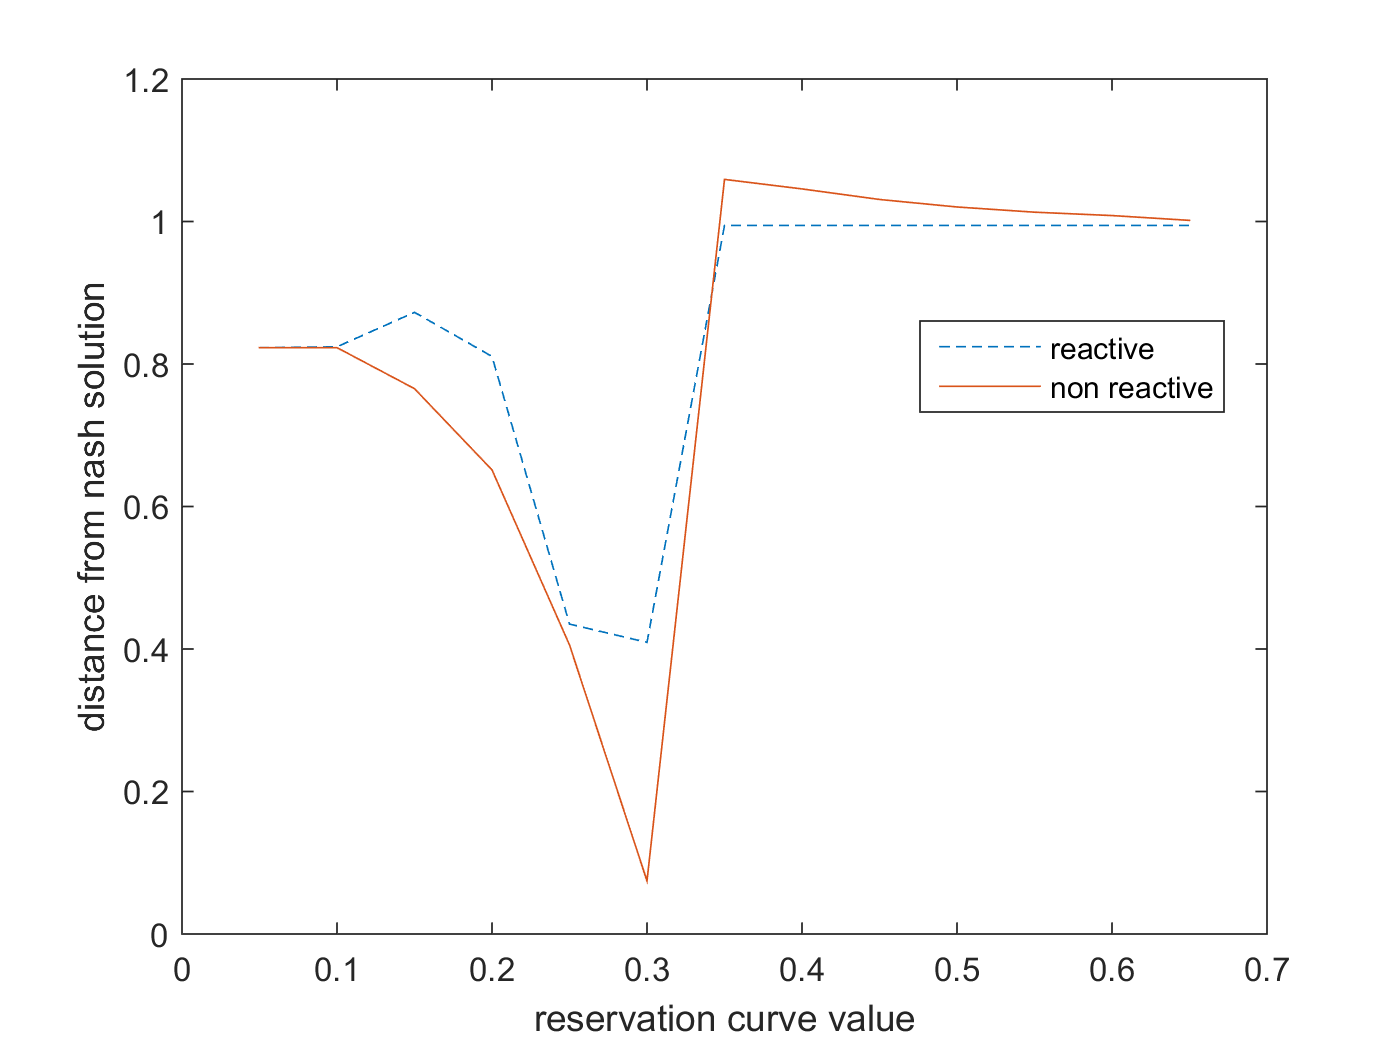
\includegraphics[width=0.7\linewidth]{img/reactivevsnonreactive}
	\caption{Distance from the Nash bargaining solution for the reactive and non reactive concession strategies. }
	\label{fig:reactivevsnonreactive}
\end{figure}

When looking at the distance and the amount of rounds necessary to find an solution (\Cref{tab:reactivevsnonreactive}), we see that although our Nash limit lies at 0.3182, this solution is not found if the reactive concession strategy is used. 

\npdecimalsign{.}
\nprounddigits{4}
\begin{table}
\begin{tabular}{|c|n{1}{4}|n{1}{4}|c|c|}
	\hline 
{{reservation utility}}	& {{distance reactive}} & {{distance nonreactive}} & {{\# of rounds}} & {{\# of rounds}} \\ 
	\hline 

0.05&0					&0					&71	&71\\
0.10&0					&0					&71	&71\\
0.15&0					&0					&75	&71\\
0.20&1.14485680268108	&0					&999	&71\\
0.25&1.16166491047958	&0					&999	&71\\
0.30&1.16559088622915	&0					&999	&71\\
0.35&1.16828500771129	&0.127686769276389	&999	&999\\
0.40&1.16753472222222	&0.279876154743691	&999	&999\\
0.45&1.16753472222222	&0.425372845848635	&999	&999\\
0.50&1.16753472222222	&0.555524071073009	&999	&999\\
0.55&1.16753472222222	&0.673260175537175	&999	&999\\
0.60 &1.16753472222222	&0.780744817700835	&999	&999\\
0.65&1.16753472222222	&0.874525088634732	&999	&999\\
\hline
\end{tabular} 
\caption{The distance in the final proposal and number of rounds of a simulation.}
\label{tab:reactivevsnonreactive}
\end{table}
\npnoround


\section{Reactive mixbed vs Nonreactive }
Although the reactive concession strategy performed worse when compared to the non reactive concession strategy, a comparison to is made when only the mixbed agent uses the reactive strategy. The mixbed agent is the most imporant agent since it ``produces'' the final demi water product.

In the comparison of the Nash Barganing Solution, in \Cref{fig:reactivevsnonreactivevsnonreactivemxbrea} it is seen that the method initially performs better than the reactive strategy. 


\begin{figure}[h]
	\centering
	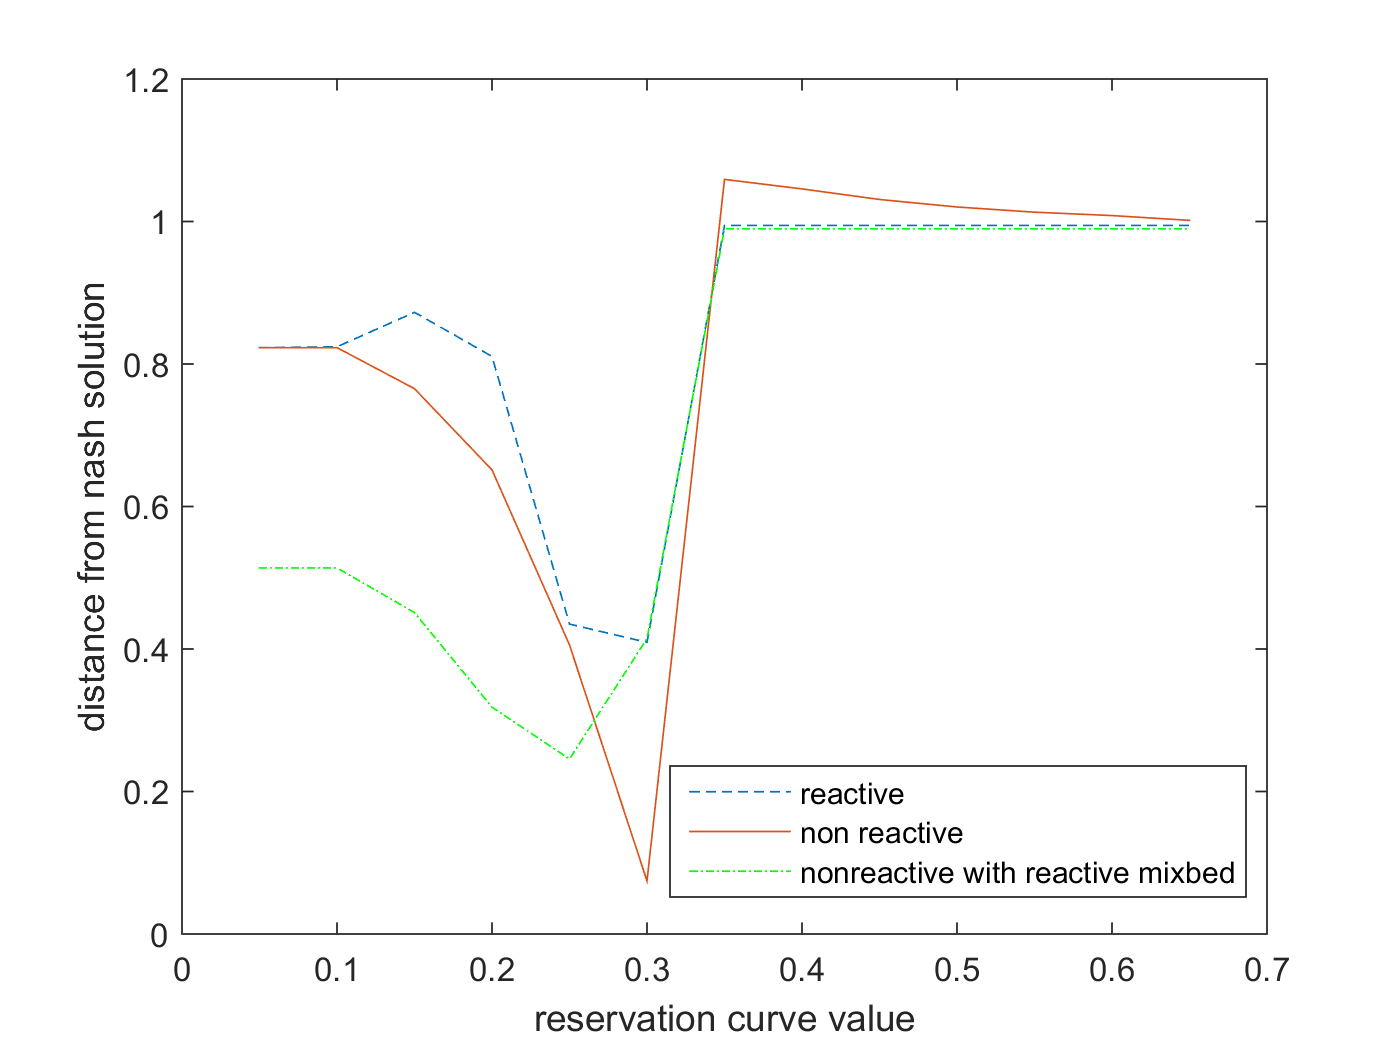
\includegraphics[width=0.7\linewidth]{img/reactivevsnonreactivevsnonreactivemxbrea}
	\caption{Comparison of the reactive and non reactive vs only reactive mixb}
	\label{fig:reactivevsnonreactivevsnonreactivemxbrea}
\end{figure}


The table of the distance and number of rounds is very repetitive. Exactly the same, although the end solution, which is the average of all offers, is close to the Nash solution. It does not find the solution within the 1000 rounds however.

\npdecimalsign{.}
\nprounddigits{4}
\begin{table}
\begin{tabular}{|c|n{1}{4}|c|}
	\hline 
	reservation utility	& {distance} & \# of rounds \\ 
	\hline 
	
	0.05&1.18691980311553 & 999\\
	0.10&1.18691980311553 & 999\\
	0.15&1.18691980311553 & 999\\
	0.20&1.18691980311553 & 999\\
	0.25&1.18691980311553 & 999\\
	0.30&1.18691980311553 & 999\\
	0.35&1.18691980311553 & 999\\
	0.40&1.18691980311553 & 999\\
	0.45&1.18691980311553 & 999\\
	0.50&1.18691980311553 & 999\\
	0.55&1.18691980311553 & 999\\
	0.60&1.18691980311553 & 999\\
	0.65&1.18691980311553 & 999\\
	\hline
\end{tabular} 
\caption{The distance in the final proposal and number of rounds of a simulation. This is where only the mixbed makes reactive concessions, and the other agents make nonreactive concessions.}
\label{tab:reactivevsnonreactivevsmixbedrea}
\end{table}
\npnoround

\section{Double water requirement mixbed}
In the design it was stated that the water ratio to the base and acid could change for the mixbed. Here an example is given where the mixbed water to base and acid ratio is 2:1:1. 

\todo[Hogere ratio pakken??]{Check for higher ratio}

\section{All}


\begin{figure}
	\centering
	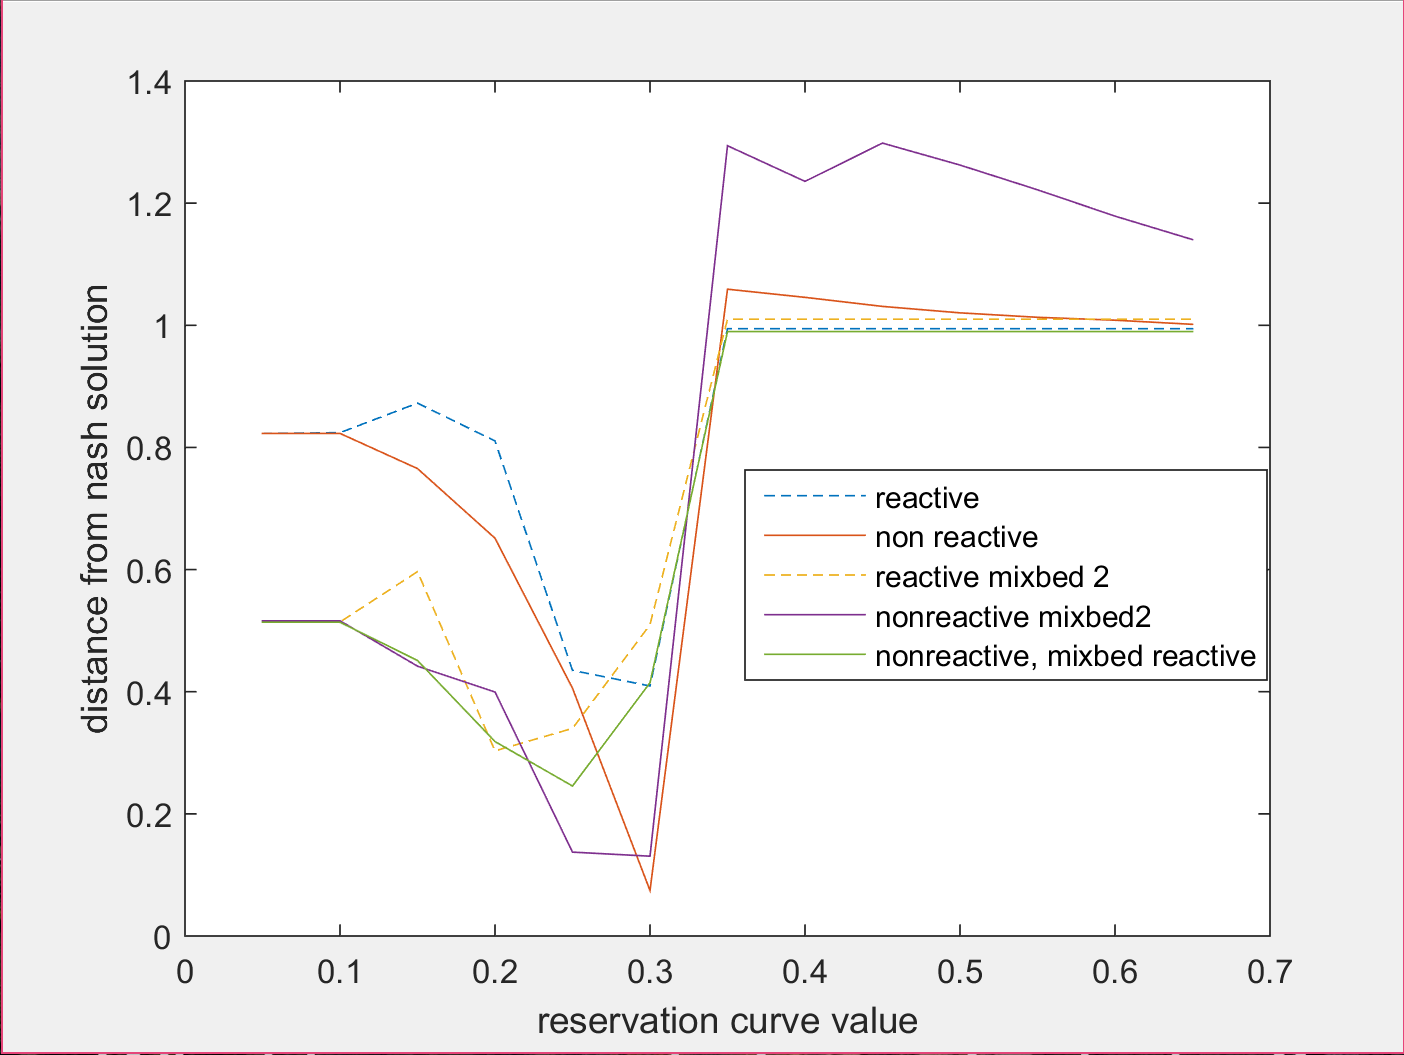
\includegraphics[width=0.7\linewidth]{img/all_dist_from_nash_solutions}
	\caption{All plots fromthe nash solutions.}
	\label{fig:alldistfromnashsolutions}
\end{figure}






\section{Discussion}
\subsection{reactive vs nonreactive}
A possible solution is that the answer can not be found as is stated by \citet{zheng2015automated} as Lemma 2. ``If Agent i deliberately stops conceding before reaching the agent's own reservation utility from time period t onward, and all other agents use the reactive concession stretegy, the negotiation will stall; i.e. other agents will reactively stop conceding and there will be no agreement, if $\Delta_j < s_j(t)-u_j(x^*_{ru_i}) and u_j(x^*_{s_i(t)})<ru_j$''.

This is although there is a nonempty zone of agreement.

\subsection{reactive mixbed vs nonreactive}
Nash solution lies in 0 water with 1 base and 1 acid. This is close to the start of mixbed in 1,1,1

This is however the result of the stalling of the mixbed, and not the result of the solution being found. This is obvious when looking at the table. Although the reservation curve changes in the offers, the mixbed does not move. This can also been seen in the proposal figure

\todo[Hier proposal figure toevoegen]{Hier proposal figure toevoegen!!}
